%% Uretildi: paper/build/submission_build.py -- elle duzenlemeyin; kaynak paper/v8/ adim dosyalaridir.
\IfFileExists{new-aiaa.cls}{%
  \documentclass[journal]{new-aiaa}
  \def\USINGAIAA{1}
}{%
  \documentclass[10pt]{article}
  \usepackage[margin=1in]{geometry}
  \usepackage{newtxtext,newtxmath}
  \usepackage{setspace}\doublespacing
  \usepackage{authblk}
  \usepackage[font=small,labelfont=bf,labelsep=space]{caption}
  \usepackage{titlesec}
  \renewcommand\thesection{\Roman{section}}
  \renewcommand\thesubsection{\Alph{subsection}}
  \renewcommand\thesubsubsection{\arabic{subsubsection}}
  \titleformat{\section}[block]{\centering\bfseries\large}{\thesection.}{0.5em}{}
  \titleformat{\subsection}[block]{\bfseries}{\thesubsection.}{0.5em}{}
  \titleformat{\subsubsection}[block]{\itshape}{\thesubsubsection.}{0.5em}{}
  \renewcommand\Authfont{\normalsize}
  \renewcommand\Affilfont{\itshape\small}
  \usepackage{cite}
}
\usepackage[utf8]{inputenc}
\usepackage[T1]{fontenc}
\usepackage{amsmath}
\usepackage{tabularx}
\usepackage{enumitem}
\usepackage{url}
\usepackage{textcomp}
\usepackage{graphicx}
\graphicspath{{../../../figures/output/}}
\makeatletter\@ifpackageloaded{hyperref}{\hypersetup{hidelinks}}{}\makeatother


\title{meryemAircraft: Tail-Sitting Blended-Wing Body for Vertical Takeoff Without Propulsor Reorientation}

\author{Meryem G\"ulmen\footnote{Independent Researcher; corresponding author, \protect\url{meryemgulmen@outlook.com}.}, Berke G\"ulmen\footnote{Independent Researcher.}, and \"Omer G\"ulmen\footnote{Independent Researcher.}}

\affil{Independent Researcher, Ankara, T\"urkiye}

\date{}

\begin{document}

\maketitle

\begin{abstract}

Hybrid aircraft for vertical takeoff and landing reach wing-borne cruise by carrying separate lift rotors or by reorienting their propulsors. This analytical study presents a tail-sitting blended-wing body arranged to change regime by rotating the airframe instead, and so carrying no mechanism that reorients a propulsor; every propulsor is a coaxial, torque-balanced pair, and a buffered series hybrid supplies the hover peak. An accounting of carried hover mass, exposed cruise drag, and hover-sized continuous power is stated first; one of its predictions holds on an independent sizing study, though not as a controlled experiment. Only the nose pair meets the accounting's escape condition; the exposed tip frames and rotors account for 57 to 69 percent of zero-lift drag. The effective lift-to-drag ratio, 5.56 to 7.39 before sizing closure, exceeds a published turboshaft quadrotor's throughout and ranges from 4 percent below to 27 percent above an all-electric one; against helicopters the result is mixed. The sizing loop closes at 52.3 to 57.5 kilograms, establishing arithmetic consistency, not that the package exists. Against lift-plus-cruise layouts the range ranking depends on the sizing contract. The buffer's required specific power is not demonstrated by the sources consulted, and the transition is not settled.

\end{abstract}



\section{The Gap}

\subsection{Two Families, Two Different Limits}

Uncrewed powered flight is dominated by two configuration families, and neither is bounded by the thing the other is bounded by.

Fixed-wing aircraft carry payload over distance efficiently, because a wing sustains the vehicle without continuously spending power on lift. Their limit is not aerodynamic but infrastructural: a runway, a catapult, or an equivalent installation.

Rotorcraft remove that requirement completely. They take off and land vertically, hover, and work from confined sites. Their limit is the converse: with no wing, every second of flight is bought with installed power, so range and endurance stay modest and worsen as the vehicle grows.

Neither family is deficient. Each is limited by the price of doing it that way. The corner where both capabilities are wanted at once is where the two applications this work is aimed at sit: wildfire observation and response, and cargo delivery to places without a runway. That corner is not empty, as the rest of this section sets out; what is unsettled is which price an architecture in it must pay.

\subsection{What the Contemporary Answers Do, and How Each Changes Regime}

Hybrid VTOL aircraft occupy that corner today. This paper does not dispute that they work. They take two routes between the regimes: lift-plus-cruise aircraft keep two sets of hardware and switch between them, and tilting aircraft keep one set and reorient it (Sec. V.A). Rotating a propulsor in flight brings a pivot and its actuators, a gyroscopic moment during the rotation, and a control problem through a regime in which the aircraft is neither a rotorcraft nor an airplane. Those are mechanical and control requirements rather than aerodynamic ones, and that distinction is what this paper is built on.

\subsection{The Third Route Is Established, and Some of Its Difficulties Are Inherited}

There is a third way to put one set of propulsors into both regimes without reorienting them: point the thrust line at the ground and let the whole aircraft rotate. The Convair XFY-1 flew it in 1954 and completed six transitions to conventional flight ``before testing was curtailed because of engine and gear-box reliability problems''~\cite{r1}, and uncrewed tail-sitters have revisited the route since. The pilot's spatial orientation and workload were real, but they are not what curtailed the testing, and they are the only ones of those documented obstacles an uncrewed aircraft removes.

Some of the difficulties were real, internal, and are inherited here. A tail-sitting vertical descent is harder than a runway landing; a tail-sitter on the ground is more exposed to crosswind; and propellers whose thrust vectors are all parallel to the body axis produce no rolling moment by any combination of thrust settings. The reaction-torque channel that other coaxial tail-sitters use about that axis is a choice this configuration declines rather than a limit it inherits (Secs. V.A and V.B).

What has changed is electric drive on each individual rotor, sensor-based attitude reference, and enough onboard computation that stability need not come from the airframe alone. The uncrewed tail-sitter literature has been exploiting exactly those three for over a decade~\cite{r2,r3}; the gap set out in Sec. I.E is not a historical one.

\subsection{What Is Already Occupied, Stated Before the Gap}

The route itself is established. Uncrewed tail-sitters combining fixed-pitch rotors with a flying wing have been built and flown for more than a decade~\cite{r2,r3}. A tail-sitter study reported in 2007~\cite{r4} already states the comparison: tilting configurations reach the same goal ``at the expense of significantly increased mechanical complexity compared to a tail-sitter that uses propeller wash over normal aircraft control surfaces to effect vertical flight control.''

Attitude without aerodynamic control surfaces is established~\cite{r3}: a quadrotor tail-sitter operated without control surfaces, with experimental verification, was reported in 2013.

Coaxial contra-rotating propulsion on a tail-sitter is established, proposed to cancel a single propeller's reaction torque without complementary controls, at a cost its proposers name as added mechanical complexity~\cite{r5}; a tail-sitting micro air vehicle reported in 2014~\cite{r6} uses a coaxial pair for the same purpose.

The established answer to hover control on such a configuration is a surface in the slipstream, and this paper refuses it. The 2014 vehicle places an elevon and a rudder in the propeller slipstream for three-axis control in hover~\cite{r6}; a flying-wing tail-sitter reported in 2018~\cite{r7} uses elevons for two of its three axes and treats the propellers' counter-moment about the thrust axis as a disturbance rather than a control channel, and reports hover and vertical flight only.

And the reaction-torque channel this paper declines is established as a control channel. A coaxial contra-rotating tail-sitter reported in 2012~\cite{r8} balances rotor torque by counter-rotation and unbalances it on purpose to steer: its published control scheme assigns ``differential velocity of the two motors'' to yaw in the vertical mode and to roll in the horizontal one. Those are the same physical channel under two names, a moment about the propeller axis, and independently driven rotors make it available to any coaxial pair. Using it is a choice, and so is declining it, which is what separates this configuration's control problem from a physical impossibility.

A blended-wing-body tail-sitter with contra-rotating propulsion, aimed at disaster response, is established, reported in 2025~\cite{r9} with vortex-lattice and RANS analysis.

A buffered series hybrid on a winged tail-sitter has been sized: a 2026 study of 100 kg winged biplane tail-sitters~\cite{r10} sizes the engine for cruise and a boost battery for vertical takeoff and landing, and gives its rotors collective pitch change mechanisms.

A coaxial tail-sitter with a series-hybrid store has been sized: a long-endurance concept reported in 2025~\cite{r11}, with a fuselage and tails, whose fuel cells charge a battery that drives the motor, because the fuel cell alone cannot fully power hover out of ground effect at takeoff; how its attitude is controlled, and whether its rotors vary pitch, the paper does not state.

And the propeller compromise at the center of this paper's own ledger is a known result, not a discovery. The uncrewed tail-sitter literature states that fixed-pitch propellers make it ``theoretically impossible to be very efficient in both hovering and forward flight.''~\cite{r2} A long-range tail-sitter reported in 2018~\cite{r2} names variable pitch as the remedy, at the cost of extra actuators and mechanism weight, and even with cyclic and collective pitch still sizes its rotor as a compromise between hover and forward flight.

\subsection{The Gap, Stated Precisely}

Each half of the required capability is well served, and both halves together are served by the contemporary hybrids. This paper does not claim otherwise. And the third route is occupied. What follows is therefore not a claim to an empty field.

What is not established is the combination taken together with its price. Specifically: a blended-wing-body tail-sitter in which every propulsor is a coaxial, torque-balanced pair (so that reaction torque and net angular momentum are given up along with the reorientation mechanism), carrying no aerodynamic control surfaces beyond a single moving device, powered through a buffered series hybrid, and audited explicitly against carried hover mass, exposed cruise drag and hover-sized continuous power, the last two of them at two scales, and under three sizing contracts.

Each of those choices costs something, and the giving-up is the part that is not free. Operating every pair torque-balanced spends the reaction-torque channel to buy the torque balance and the near-zero net angular momentum, and leaves the moment about the propeller axis to a single aerodynamic device.

None of the elements is new, and Sec. V.A says so. Tail-sitting aircraft are seventy years old~\cite{r1}; blended wing bodies have been a standing subject of transport research for more than three decades~\cite{r12}; series-hybrid propulsion has been designed for small uncrewed aircraft~\cite{r13}. The route is not claimed to have been waiting to be found. The contribution is the architecture: a configuration arranged to change regime by rotating the airframe rather than its propulsors, and so carrying no mechanism that reorients a propulsor. The combination, the consequences of the choices inside it, and an accounting of what they cost are how that contribution is presented and priced.

\section{The Charges, the Condition, an Independent Check}

\subsection{The Tax}

A claim that one architecture escapes a cost shared by the others is only meaningful if the cost is stated first, in terms that do not presume the escape. This section states it. It is not a claim about any particular aircraft, and nothing in it is new physics; what it provides is the accounting that the rest of the paper is checked against.

\subsubsection{The Root: A Duty Cycle That Does Not Match the Hardware}

For a mission of one hour, a takeoff, a transition, a return transition and a landing occupy on the order of a minute, roughly two percent of the flight. An architecture that provides the vertical phase with a dedicated lift subsystem therefore carries it for fifty times as long as it uses it. This is not an implementation defect and it cannot be removed by making the subsystem better, because it is a statement about duty cycle rather than about quality. The mismatch between how long a component is needed and how long it is present is the origin of all three charges that follow.

The statement is deliberately confined to architectures with a dedicated lift subsystem, because that is the family the charges describe.

\subsubsection{Bill 1: Mass}

A lift-plus-cruise aircraft carries two propulsion groups: rotors, motors, mounts, wiring and structural reinforcement for the vertical phase, and a separate propulsor for cruise. The vertical group provides no required lift or thrust during cruise and is lifted anyway.

Its cost is not linear. Mass growth feeds itself ($\mathrm{MTOW} = m_\mathrm{payload}/(1 - f_\mathrm{empty} - f_\mathrm{energy})$ puts additional empty mass through a multiplier that grows as the denominator shrinks), and in the vertical phase the same increment is counted a second time, because at a fixed disc area hover power scales with W\^{}1.5. A modest dead-mass fraction becomes a large payload penalty.

\subsubsection{Bill 2: Drag}

The second payment falls on architectures that leave hover hardware exposed in forward flight: rotors stopped in the airstream, the booms that carry them, and the interference between their wakes and the wing. Cruise drag has other sources on any aircraft; what is charged here is the part attributable to hardware retained for a phase that is over.

Wind-tunnel work on a hybrid airframe found that the difference between propellers parallel to the airflow and no propellers at all is modest, while ``the drag produced by the motors is significant.''~\cite{r14} The bill is charged mainly by the motors: hardware that cannot be feathered or aligned away, because its cost is its presence; the same work notes that its motors were chosen for performance rather than for low drag, and that the drag of the supporting beams is limited. Wind-tunnel characterization of a quadplane found drag in the hybrid regime generally exceeding either pure mode through adverse flow interaction, and that a simulation assuming negligible rotor--structure interaction ``always predicts higher lift and lower drag than were experimentally observed.''~\cite{r15}

The important property of this charge is not its size but where it falls. It is charged per unit time in cruise, so it grows with exactly the quantity the aircraft exists to maximize.

\subsubsection{Bill 3: Power System Sizing}

A VTOL aircraft must install enough power to hover. The ratio between the two demands follows from the governing equations rather than from any design choice (Supplement S2):

\begin{equation}
\frac{P_\mathrm{hover}}{P_\mathrm{cruise}} = \sqrt{\frac{DL}{2\rho}}\,\frac{L/D}{V}\,\frac{\eta_p}{\eta_h}
\end{equation}

The quantities on the right come from the configuration and from the propulsion operating points, not from the duration of the hover phase. $\eta_h$ and $\eta_p$ are not configuration constants, they depend on the propeller and on the condition it is run at, and Sec. VI.B computes what happens when one fixed-pitch blade has to supply both. Raising the disc loading raises the ratio as its square root.

The power system is therefore sized by a condition that holds for a minute and is then carried, unused, for an hour. Sizing by hover means an oversized engine, or a battery that must deliver a peak it will rarely be asked for, or both, and whichever is chosen, the extra installed capacity is mass: a cost in kilograms, though not Bill 1.

\subsubsection{The Charges Are Coupled: Remedies Move Cost, Among the Three Charges or Outside Them}

The three charges are not independent problems with independent fixes. Each known partial remedy reduces one charge and pays for it, in another charge or in a cost outside the three. They are three distinct accounting quantities, paid in kilograms, drag counts and installed kilowatts, and they are not assumed to be independent physical causes: a remedy can move a requirement from one currency into another. Whether a change of size moves them together, which would make them one quantity under three names, is tested in Sec. VI.C.

A charge and its currency are not the same thing. Each charge is one specific payment, not the name of the currency it is paid in. Bill 1, as this accounting uses it, is the mass of a dedicated lift subsystem; Bill 2, the cruise drag of hover hardware left exposed; Bill 3, continuous power installed to a hover peak.

\begin{table}[htbp]
\centering
\caption{Known partial remedies and the charges they move}
\label{tab:1}
\small
\begin{tabularx}{\linewidth}{XXX}
\hline
Move & Bill it attacks & What it creates (a bill by its number, any other cost in words) \\ \hline
Distributed electric lift rotors & 3: the cruise engine no longer sizes to hover & 1 and 2: many rotors and mounts, permanently carried and exposed \\
Folding or retracting lift rotors & 2: the exposed rotor is removed from cruise & 1: mechanism, actuation, locking; and a new failure mode, not among the three \\
Tilt-rotor, tilt-wing, tilt-nacelle & 1: one propulsion group serves both regimes & kilograms, not Bill 1: the pivot and its actuators; Bill 3, imposed or left standing according to how the architecture the move modifies supplies its hover peak (with no store, the power plant is sized by the hover peak); and gyroscopic coupling and a transition control problem, which are not among the three \\
Variable-pitch or feathering propulsors & 1 and 3: one propulsor is retrimmed across two widely separated operating points instead of duplicated & kilograms, not Bill 1: pitch hub and actuation; and a new failure mode, not among the three \\
Higher disc loading, smaller rotors & 1 and 2: smaller, lighter, cleaner rotors & 3: hover power rises with $\sqrt{DL}$ \\
Lower disc loading, larger rotors & 3: hover power falls & 1 and 2: larger structure and exposed area \\
\hline
\end{tabularx}
\end{table}

One row pays part of its cost in none of the three currencies, and that is not an oversight: the tilting row's gyroscopic coupling and transition control problem are costs, but not charges this accounting tracks. Table 1 is not a census of the field; it lists the moves whose transfers are documented, and a remedy absent from it is not thereby claimed to cancel a charge.

One of these transfers has direct experimental support~\cite{r14} (Supplement S2).

\subsubsection{What This Accounting Is For}

The accounting is refuted by a counter-example, and Table 1 is where one would appear: every entry in it moves cost rather than removing it.

Stated positively, so that the test can actually be run: a counter-example is a remedy that reduces one of the three charges, leaves the other two no worse, and whose own cost is either absent or demonstrably smaller than the reduction, measured in the same currency. The accounting claims transfer. It does not claim that every architecture is equally good, and a remedy that is simply a better bargain in one currency refutes it.

Two clarifications keep the test from being either too easy or unfalsifiable. ``No worse'' is judged against the architecture the move modifies. A move that reduces one charge and makes another worse is a transfer between charges. And a remedy whose cost falls outside the three charges does not refute the accounting, because the accounting is about those three; but it is not thereby exempt from being counted. The tilting row, which needs both clarifications, is worked through in Supplement S2.

The accounting also makes a prediction that can be checked without settling the architectural question at all: where an arrangement pays one charge heavily in order to escape another, its ranking against a differently-balanced arrangement will move when the sizing rule changes (toward the lighter arrangement as the rule weights mass more) and will reverse where that reweighting carries it past the point at which the two break even. Section VI.D tests both the movement and the reversal on this configuration, and Sec. II.C tests a different consequence against a sizing study this work did not produce.

Whether an architecture can decline the mismatch itself, rather than redistribute its consequences, is a different question, and the next section states the condition it would have to meet.

\subsection{The Escape Condition}

This section asks what an architecture would have to do in order not to incur the three charges at all. The answer is a definition, derived by inverting Table 1, and it is stated here before any configuration is offered so that the standard is not taken from the thing it will be used to measure.

\subsubsection{Inverting the Table}

A charge appears wherever the two regimes are served by hardware that departs from one of four things: the same hardware, serving both duties, held in one orientation, with the hover peak supplied other than by its continuously installed power. Different hardware costs Bills 1 and 2. The same hardware serving only one duty costs them again. The same hardware serving both duties in a different orientation is the tilting family. The same hardware, both duties, one orientation, but a different sizing point incurs Bill 3. What each departure costs is in Supplement S3. Read one at a time, these are ways to pay. Read as a conjunction, they are a condition.

\subsubsection{The Condition}

\begin{quote}
An architecture does not incur the three charges if the propulsors that carry the weight, held in one orientation relative to the airframe, produce both the hover thrust and the cruise thrust, and if the difference between the hover peak and the cruise demand is supplied from a store rather than from permanently installed continuous power.
\end{quote}

Four parts: same hardware, both duties, one orientation, hover peak from a store.

Two things in that sentence are choices rather than derivations. The inversion requires only one orientation relative to the airframe; how an architecture keeps that while changing flight regime (by rotating the whole body, or otherwise) is not in the inversion, and is treated as exposition rather than as part of the definition. And the fourth departure's exception lets the peak come from any source other than the continuously installed power; a store is the narrower reading used here, because it is what the configuration examined later uses and because a narrower condition is easier to fail.

\subsubsection{What the Condition Does Not Say, and This Matters More than What It Says}

It means zero of the three charges as Sec. II.A defines them. It does not mean an architecture that costs nothing, and it does not mean an architecture that carries nothing for the vertical phase. A definition that placed every conceivable cost inside the thing to be escaped would be unfalsifiable. Six costs are permitted, named here before any candidate is examined (the working is in Supplement S3):

\begin{enumerate}[label=\arabic*)]
\item A store is permitted, though it is mass carried for a duty that is briefly needed, which is the complaint Bill 1 makes. It does not claim the trade is favorable: whether the store is lighter than the continuous power it displaces is computed, not asserted.
\item Releasing the engine is not releasing the electrical path. Machines, power electronics and wiring still pass the full hover power, and that Bill 3 is carried in the ledger.
\item Rotating the airframe is permitted and is not priced here. An architecture that rotates its whole body still turns its thrust axis through ninety degrees relative to the flight path, with the moments and the control through the turn that implies; that is not one of the three charges, and Sec. VI.A analyzes the transition without pricing it.
\item Hardware installed for the vertical phase is permitted if it serves both duties.
\item Hardware used in both regimes for something other than propulsive thrust is permitted, and its cruise drag is not eliminated. Cruise thrust in this paper means the thrust that balances cruise drag. Attitude devices produce none; used throughout the flight, they fall outside Bill 1, and they do not stop the propulsor that carries the aircraft from meeting the condition. But carried through cruise without producing cruise thrust, they are the first failure mode that follows, and Bill 2 reaches them.
\item Serving two regimes with one set of hardware has a price of its own: a fixed geometry cannot be optimized for both, and the compromise is paid in efficiency. The condition permits that cost and does not measure it. Section VI.B does.
\end{enumerate}

One exclusion, stated narrowly. Structure, surfaces and actuation present for reasons other than the vertical phase are not charged as duty-cycle mismatch under this accounting, which says which ledger they belong in, not that they are free; it does not reach a part that would not exist but for the vertical phase. The tip frames of Sec. III are landing gear because the aircraft stands on its tail: their mass is charged in the build-up and their drag in the ledger.

\subsubsection{The Condition Can Fail, and How}

An architecture fails the condition if any of the following holds:

\begin{enumerate}[label=\arabic*)]
\item It carries a propulsor through cruise that produces no cruise thrust.
\item It changes the orientation of a propulsor relative to the airframe in order to change regime.
\item Its continuously installed power is sized by the hover requirement rather than by cruise.
\item It satisfies the first three only in part (for instance in its primary propulsor while a secondary set fails them), in which case the instantiation is partial, and the part that fails re-opens the charge it fails.
\end{enumerate}

\subsubsection{What Follows from the Condition, and What Does Not}

The condition is a statement about what an architecture would have to be. It is not a claim that anything satisfies it, not a claim that anything satisfying it would fly, and not a claim that satisfying it is desirable.

An architecture that reorients a propulsor does not satisfy the condition as written, because the condition requires one orientation relative to the airframe. Whether such an architecture might avoid the three charges by some other route is a separate question this paper does not settle; the condition is a definition, not a law, and it can be too narrow without being wrong.

\subsection{An Independent Quantitative Check}

An accounting proposed by the same people who then use it invites one obvious objection: that the charges were chosen because a particular aircraft happens not to pay them. What follows is not a test of the whole framework. It checks one falsifiable consequence on one independent data set. The working is in Supplement S4.

The prediction has two halves, and only the first is a derivation.

\begin{quote}
First half, derived from Sec. II.A. A configuration carrying a dedicated lift system pays for it in gross weight, and the payment is amplified.
\end{quote}

\begin{quote}
Second half, not derived. That the cruise efficiency the arrangement buys does not cover that payment.
\end{quote}

The check tests the second half on independent data, with the first half supplying the reason to expect the outcome: the weight charge is amplified by a multiplier, while the efficiency credit enters linearly through the cruise lift-to-drag ratio. The prediction is also mission-dependent, and the page would be weaker for hiding it. The mass charge of carried lift hardware is roughly fixed; the efficiency credit accumulates with distance. The mission used here is short.

The check uses a NASA study~\cite{r16}, conducted for its own purposes and with no relationship to the present work, that sizes five VTOL architecture families (nine designs in all) against a single mission with common tools and common assumptions; it does not use the three-bill accounting of Sec. II.A or any framework derived from it. It is used for three reasons, stated so that the choice is not merely the one that agreed: it holds the mission fixed across architecture families, it applies one set of tools to all of them, and it reports both quantities this prediction needs. The mission is 1200 lb of payload over 75 nautical miles. Two of the nine designs matter here. The turbo-electric lift-plus-cruise design reaches 8.5 at 7271 lb and carries a dedicated lift group: eight lift motors beside its cruise motor. The turbo-electric tilt-wing reaches 8.6 at 6584 lb with none: eight proprotors, reoriented.

The primary comparison is the lift-plus-cruise design against the tilt-wing, because they isolate the charge: they share the mission, the payload, the turbo-electric propulsion architecture and the presence of a cruising wing. They are not identical in every other respect (one stops its lift rotors in the airstream and drives a separate pusher, the other reorients its proprotors on a tilting wing), but the difference the comparison turns on is that one carries a dedicated lift group through cruise and the other does not. The comparison is the closest the published set comes to isolating that charge; it is not a controlled experiment. The tilt-wing is 1.2\% better in effective cruise efficiency and 9.4\% lighter. The design gross weights differ by 687 lb in the tilt-wing's favor. That figure is the net difference between two architectures, not the measured mass of a lift group. The published weight breakdown is consistent with the transfer property of Sec. II.A (the mechanism giving part of the structural saving back) inside a breakdown this work did not produce: its three reported categories account for 580 lb of the 679 lb empty-weight difference, and the remaining 99 lb lies in categories it does not break out (Supplement S4). The framework does not predict any of these numbers; without the input fractions it predicts no magnitudes. What it predicts is that the amplified weight charge survives the efficiency credit, and on the isolated pair it does so with the credit reduced to nothing.

The architecture proposed later in this paper is not the only way to avoid the first charge. The tilting family avoids it too. The margin in cruise efficiency is 0.1 in effective lift-to-drag ratio, and nothing is claimed from its direction. What separates the tilting family from the configuration described later is not this axis; it is what each pays, and a sizing study does not settle that.

The check establishes that one prediction of the accounting holds on data produced elsewhere, for purposes unrelated to this argument. It does not establish that the accounting is complete, that the three charges are the only costs an architecture pays, or that avoiding them makes an aircraft better. It does not establish anything about the configuration this paper proposes, which has not yet been described, and which is not in the study used here. An instrument whose first use is to measure the thing its authors are advocating should be shown working on something else first, and that is why this section comes before the aircraft. The instrument is now fixed, and it is not modified again. Everything that follows is measured with it rather than added to it.

\section{The First Half: Operation Without a Runway}

\subsection{The Opponent, and the Axis}

On this axis the alternative is the fixed-wing aircraft, and the comparison runs one way only. Nothing here is claimed against fixed-wing aircraft on range or cruise efficiency, where a runway-launched airplane that never bought vertical capability pays none of the charges of Sec. II.A and is the better machine. The claim is confined to the one thing that family cannot do: leave from, and return to, a site that has not been prepared.

\subsection{What the Requirement Actually Is}

A catapult-launched fixed-wing aircraft also leaves without a runway. What it does not do is come back to the same unprepared site, and it does not travel without the launcher. The two applications this work is aimed at need the aircraft to arrive somewhere that has no infrastructure, and to leave again.

So the requirement is: the aircraft carries everything it needs to depart and recover, and the site supplies no prepared launch or recovery infrastructure of any kind. A net, a catapult, a cradle, a prepared strip or a recovery vehicle each fail that test, including the ones that fail it only on the recovery half.

\subsection{How the Configuration Meets It}

The aircraft stands on its tail, with its longitudinal axis vertical, in its own storage attitude (Fig. 1). No launch equipment is present. It rests on five points: the four lower ends of the tip frames and the aft end of a keel running along the centerline.

\begin{figure}[htbp]
\centering
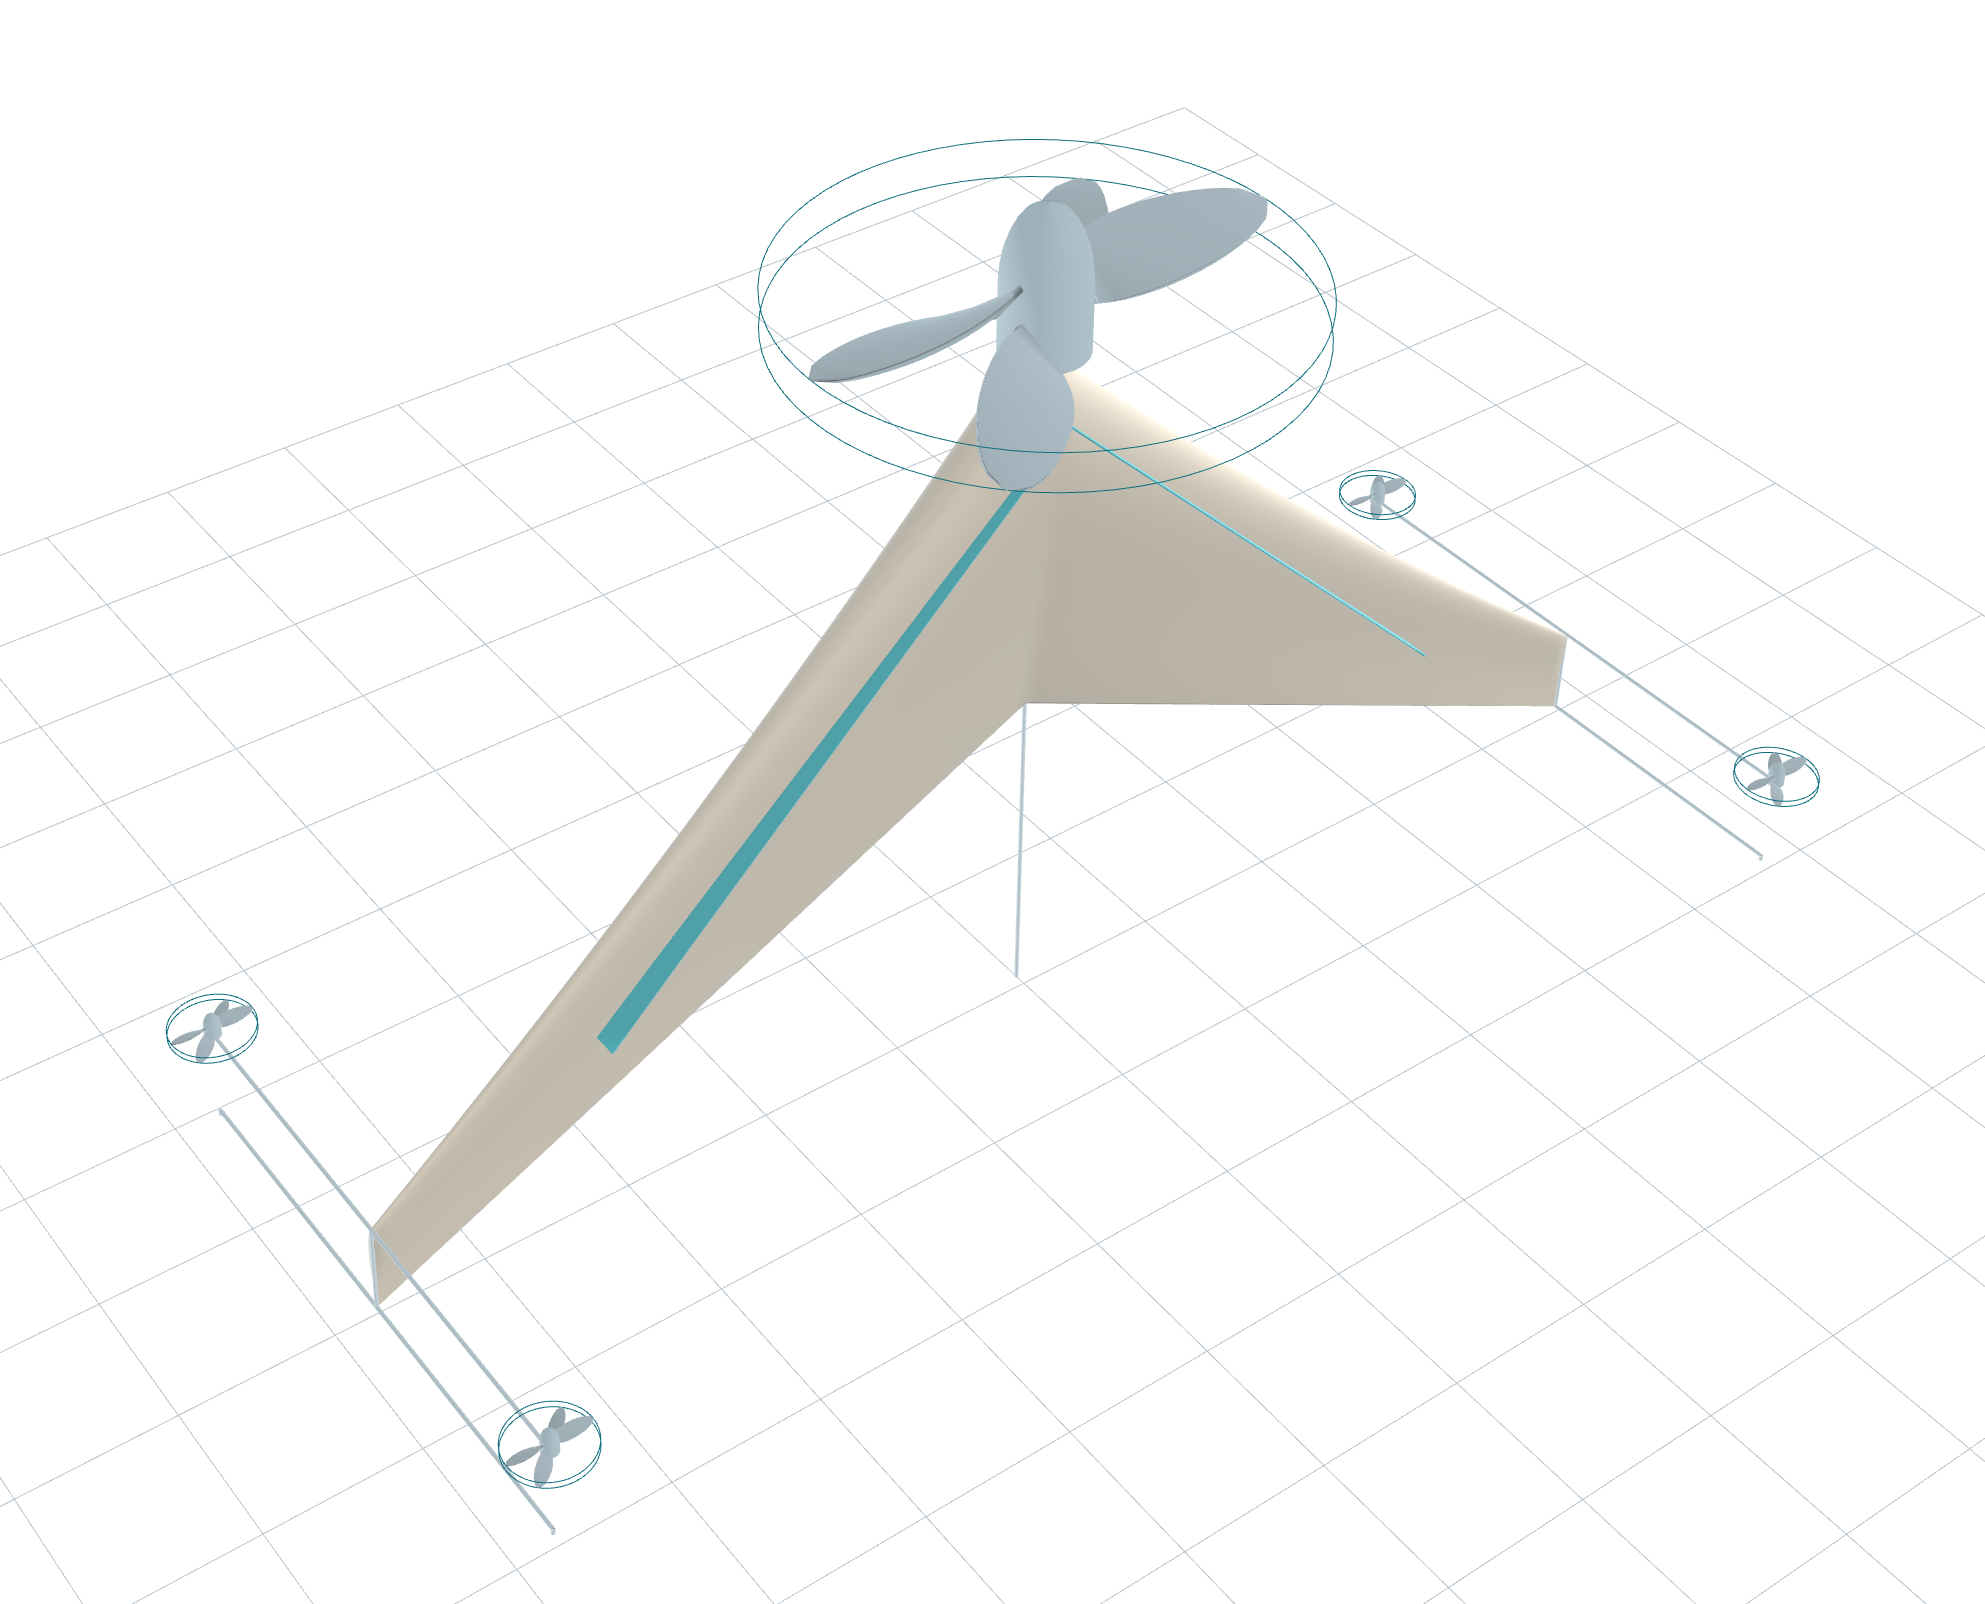
\includegraphics[width=0.75\linewidth]{v8-f1-standing.png}
\caption{The 50 kg reference design standing on its tail: nose pair uppermost, tip frames and keel on the ground, strip on the lower surface; blades schematic}
\label{fig:1}
\end{figure}

Those five points are not added hardware. The tip frames are the landing structure, they are also the structure that carries the four tip pairs (the attitude propellers) and sets their moment arm, and their fairing is the aircraft's only vertical surface. One structure serves four purposes and is charged to the mass budget once; Sec. V.B gives the fairing's sizing.

The saving has precedent and it is not this paper's observation. Reviewing the tail-sitters of the 1950s, NASA recorded~\cite{r17} that ``dispensing with a conventional landing gear improved the empty weight fraction for these VATOL aircraft'', while noting that some form of gear was still required on the tail surfaces, that such gear was limited to low sink rates, and that tip-over was ``a constant worry in gusty air and on uneven ground, particularly with the propellers turning.'' The present arrangement takes the weight benefit and extends it by giving the same structure the control duty as well.

And the stance base is a parameter rather than a constraint. Moving the frame ends further outboard widens the base against ground wind without altering the planform, the propulsion or the control architecture, and because the same displacement lengthens the control moment arm, both benefits arrive from one change. The 50 kg reference geometry (Sec. V.B) is one point on that trade; an operator with a stronger ground-wind requirement can take another.

\subsection{What Is Sized, and What Is Not Demonstrated}

Sized. The vertical phase is sized: hover power from momentum theory at thrust equal to weight, the buffer that supplies what the engine cannot deliver of that peak (at a specific power Sec. VII examines), the tip-frame lengths that set both the stance base and the control arms, and the structure that carries the landing loads. Section VI.A reports whether they close. This section does not assert the outcome of a calculation it does not contain.

Not demonstrated.

The aircraft leaves the ground on its tip pairs. The nose pair is sized at thrust equal to weight, so the takeoff margin comes from the four tip pairs, which were sized from the moment requirement. That is the one place the configuration asks a component to do a second job it was not sized for, and it means the takeoff margin and the attitude authority are drawn from the same propellers and compete for it.

The vertical descent and the landing transition have not been analyzed. Whether the descent enters the vortex ring state is an open question in Supplement S14; the landing transition is not the takeoff transition run backwards, and no figure in this paper describes it (Supplement S5).

Hover attitude control is sized but not demonstrated as a closed loop: the moments about each axis are computed, and no control allocation has been closed around them. This configuration also declines the reaction-torque channel that comparable aircraft use about the body's longitudinal axis (Sec. V.B). What that refusal costs in authority and in response time is not computed, and Supplement S14 carries it.

And one historical difficulty is inherited rather than removed. A tail-sitting aircraft on the ground is more prone than a conventional one to tip over, in crosswind and on uneven ground. The stance base is the answer this configuration offers, and it is a parameter rather than a proof.

\subsection{What the Historical Record Does and Does Not Give Back}

One of the 1954 objections is genuinely removed and it should be named exactly. The landing difficulty of the 1950s tail-sitters was attributed~\cite{r17} to a pilot judging a backwards vertical descent by looking over his shoulder, to turbulence sensitivity and to reduced control power near touchdown. There is no pilot here, and height above ground is a sensor measurement rather than a human estimate. That disposes of the spatial-orientation objection and nothing else. Precise hovering, ground gusts and the descent itself are not disposed of by removing the pilot, and this section does not pretend otherwise.

\subsection{What This Half Costs}

Runway independence is not obtained free, and the charges appear later rather than here. The tip frames that make the aircraft self-supporting are structure standing in the cruise airstream, and Sec. VI.B charges their drag. The tip pairs they carry are exposed for the whole cruise and cannot be feathered, and Sec. VI.B charges that too. The buffer that releases the engine from the hover peak is mass carried for the whole flight.

The second half (cruise carried on a wing rather than on rotors) is the subject of the next section, and the two are combined in Sec. V.A.

\section{The Second Half: Cruise Carried on a Wing}

\subsection{The Opponent, and the Axis}

On this axis the alternative is the rotorcraft (multirotor and helicopter alike), and as in the previous section the comparison runs one way only. Nothing here is claimed against fixed-wing aircraft. The claim is confined to the one thing the rotorcraft family structurally lacks: a surface that carries the cruise lift.

\subsection{What the Requirement Is}

Section III established the first half: the aircraft must leave from and return to a site that supplies nothing. A rotorcraft meets that requirement completely.

What it does not meet is the second half of both missions. Wildfire observation and response, and cargo delivery to places without a runway, each require the aircraft to cover distance after it has left the unprepared site, and a vehicle with no wing buys every second of that distance with installed power. The consequence has been stated independently: surveying the field, one study concludes~\cite{r18} that multirotors are efficient in hover and suited to short-range missions, while vectored-thrust aircraft are efficient in cruise and suited to long-range ones.

\subsection{What the Configuration Does Instead}

Cruise lift is carried by the airframe itself. At the cruise condition the lift coefficient follows from $C_L = W/(qS)$, the drag from $C_D = C_{D0} + C_L^2/(\pi A\!R\,e)$, and the nose pair is left with one job: producing the thrust that balances that drag. It supports none of the weight.

A rotorcraft's rotors must produce the lift and the propulsive force together, throughout cruise. This aircraft separates them: a surface holds the aircraft up and a propeller pushes it along, and the wing produces its lift without a separate continuous power supply of its own; the power the aircraft spends in cruise goes to overcoming drag, of which the lift's share is the induced part.

But the size of the resulting advantage is a calculation, not a consequence of that statement. The rest of this section is the calculation, and it gives a smaller number than the structural statement invites.

\subsection{What the Margin Actually Is, in One Currency}

The sizing set of Sec. II.C reports~\cite{r16} an effective lift-to-drag ratio, $(L/D)_e = WV/P$: a system figure of merit that already contains the propulsive efficiency of whatever produces the thrust, so a force ratio cannot be placed beside it. In level cruise, with shaft power $P = DV/\eta_p$,

\begin{equation}
(L/D)_e = \frac{WV}{P} = (L/D)\,\eta_p
\end{equation}

Which power $P$ denotes is not assumed here, because reading it as electrical rather than shaft power would make this configuration's figure incomparable with the published one. The source writes hover power~\cite{r16} with the figure of merit applied, which is shaft power, and applies the propulsion-system efficiency separately, for the all-electric entries as for the shaft-driven ones.

The aerodynamic ratio is 8.79 to 10.82, with the tip frames and the free-wheeling tip-pair rotors (Sec. V.B) already charged; that spread is uncertainty, the zero-lift drag bracket. The cruise propeller efficiency is 0.632 to 0.683 across the nose-blade families that meet the hover figure of merit; that spread is not uncertainty but a design variable this study has not fixed (Table 2).

\begin{table}[htbp]
\centering
\caption{Effective lift-to-drag ratio at the corners of the drag and propeller-efficiency brackets}
\label{tab:2}
\small
\begin{tabularx}{\linewidth}{lrr}
\hline
$(L/D)_e$ & $\eta_p$ 0.632 & $\eta_p$ 0.683 \\ \hline
L/D 8.79 (adverse drag) & 5.56 & 6.00 \\
L/D 10.82 (favorable drag) & 6.84 & 7.39 \\
\hline
\end{tabularx}
\end{table}

These are the bounding corners of a product, not four simulated aircraft. Across the examined envelope they give 5.56 to 7.39; for the best examined blade family, at 0.683, 6.00 to 7.39. Which blade a designer would choose also turns on structural loads, acoustics, the motor operating point, rotor inertia and manufacture, none of which is modeled in this work (Supplement S6). Section VI.A carries one blade into a closed sizing loop; until then no corner is presented as the aircraft's performance.

\subsection{What the Comparison Gives, Against Both Published Quadrotors}

The sizing set contains two quadrotors for the same mission (Table 3), and neither is treated here as the primary one.

\begin{table}[htbp]
\centering
\caption{Effective lift-to-drag ratio against the two published quadrotors}
\label{tab:3}
\small
\begin{tabularx}{\linewidth}{XrXX}
\hline
 & $(L/D)_e$ & vs examined envelope 5.56 -- 7.39 & vs best examined family 6.00 -- 7.39 \\ \hline
Quadrotor, turboshaft & 4.9 & +13\% \ldots{} +51\% & +22\% \ldots{} +51\% \\
Quadrotor, all-electric & 5.8 & $-$4\% \ldots{} +27\% & +3\% \ldots{} +27\% \\
\hline
\end{tabularx}
\end{table}

Against the turboshaft quadrotor the sign holds at every corner of both readings; closing it would need a propeller efficiency of 0.557, against 0.632 for the least efficient blade family examined.

Against the all-electric quadrotor it does not hold at the low corner, and that result is reported as a result rather than as a caveat. That vehicle reaches 5.8 with 1742 lb of battery and nearly twice the gross weight for the same mission, 7221 lb against 3678 lb. That higher gross weight is consistent with the mass charge Sec. II.A describes; Table 3 alone does not establish the causal link, and Sec. II.C sets out the independent evidence for it.

The same sizing set gives four entries for its two helicopter types, at 5.4 to 7.2, and against them the result is mixed: this configuration is ahead of the turboshaft single-main-rotor helicopter at every corner, the two middle entries fall inside its envelope, and only its top corner is ahead of the all-electric side-by-side helicopter, which has no wing either. The qualifications that follow apply to them too.

So the second claim is narrower than the structural statement invites: carrying cruise lift on a wing is worth roughly an eighth to a half against the turboshaft reference, and against the all-electric one it ranges from slightly behind to comfortably ahead depending on the drag outcome and the blade: a measurable advantage, not a change of category. What compresses it is the cruise efficiency of the fixed-pitch blade: at a propeller efficiency of 0.85 the same airframe reaches 7.47 to 9.20. Whether a variable-pitch hub would recover that difference is not computed; Sec. VI.B reports the gap and declines to attribute all of it to the hub.

\subsection{Five Qualifications: Three Run Against This Configuration, One Has No Computed Direction, and One Bounds What the Comparison Can Be Called}

Scale. The compared vehicles are larger than both designs studied here, which are of order 50 kg and 1000 kg (Supplement S6), and Reynolds number favors the larger aircraft, so the smaller design is at a disadvantage in this comparison rather than an advantage.

The quadrotor is a good quadrotor: both quadrotors have unusually low disc loadings. Nothing here is compared against a poor example.

The speeds are not matched, and the direction of that mismatch is calculable. The reference is quoted at its best-range speed, this configuration at its cruise condition, 1.49 times stall, rather than at its best point, 1.26. The reference is therefore given its best speed and this configuration is not given its best speed, and the margin is positive anyway. The best point is not an available option (cruising there leaves too little margin above the stall), so this fixes a direction, not a magnitude.

The atmospheres are not matched. The published sizing mission is flown at ``5,000-ft altitude and ISA + 20$^\circ$C''~\cite{r16}; every number in this work is at sea level. The direction of that mismatch is not claimed here, because it has not been computed.

The analysis chains are not matched, and this is the qualification that bounds what the comparison can be called. The published value comes from a fully sized vehicle in an integrated design system; the value here is a converted metric at a prescribed cruise condition, taken before the sizing closure of Sec. VI.A. So this is a comparison of two independently produced figures in a common definition, not a controlled numerical reproduction, and nothing in it should be read as validation of either, or as a completed aircraft-level comparison.

\subsection{What Is Sized, and What Is Not Demonstrated}

Sized. The drag build-up and its bracket, the lift-to-drag ratio from the drag polar, the propeller efficiency from blade-element momentum theory, with section polars from NeuralFoil 0.3.3~\cite{r19}, at two operating points, and the range that follows from the chain.

Not demonstrated. No part of this has been measured: there is no wind-tunnel or flight test in this work, and the drag coefficient is a build-up with a declared bracket. The planform was chosen rather than optimized. The span efficiency used throughout this section is the computed value, 0.817, not the assumed 0.85, from a vortex-lattice solution (AeroSandbox 4.2.10~\cite{r20}) of the trimmed planform. And for the methods used here, and for the published comparisons against which they were checked, the aerodynamic predictions diverge above roughly ten degrees of incidence: three methods of three fidelities depart at the same place, the highest of them against wind-tunnel measurement~\cite{r21,r22}. That is a statement about these methods on this class of configuration, not about what any method could achieve; it does not touch the preceding cruise numbers, which sit at a few degrees, but it bounds what this section may be read to support, and the transition of Secs. V.A and VI.A passes through that band.

\subsection{What This Half Costs}

The wing that makes cruise efficient is carried through the vertical phase, where it produces nothing and presents the aircraft's largest surface to ground wind; the tailless planform constrains the sweep; and the fixed-pitch propeller is why the preceding margin sits where it does. Section VI.B charges the third. The first two are inside Sec. VI.A's closed numbers but are not separated out as charges, and the wing's exposure to ground wind is not priced in this work.

The two halves are now on the table separately. Section V.A is where they are combined, and the combination is what this paper is for.

\section{Combining the Solutions}

\subsection{The Combination}

None of the three elements is new. Each can be found on its own, and some of them together, in the literature and in hardware; Sec. I says where. The principle behind the third element (a continuous plant sized for cruise, with the vertical or takeoff peak drawn from a store) has been applied in studies of a winged tail-sitter (Sec. I)~\cite{r10} and of a single-aisle airliner reported in 2016~\cite{r23} whose turbines are ``sized for efficient operation during'' cruise and assisted by electric motors ``during takeoff and climb.''

What this paper contributes is the architecture that brings the three elements together; the condition shows what it satisfies, and the price shows what it costs. The three elements, taken together, meet the escape condition of Sec. II.B in the propulsor that carries the aircraft, and they meet it with no mechanism that reorients a propulsor. The assembly is not offered as novel because it is an assembly. It is offered for what it satisfies, and for what it does not need in order to satisfy it.

The qualification ``in the propulsor that carries the aircraft'' is not decoration. The single nose pair meets all four parts of the condition. The four tip pairs do not: they are exposed in the cruise flow and cannot be feathered, so they re-open the second charge. The instantiation is therefore partial, the case Sec. II.B lists among the ways to fail, and reporting what the failing part costs is a substantial share of what Sec. VI.B does.

Each element supplies one part of the condition, and none supplies it alone:

\begin{enumerate}[label=\arabic*)]
\item The blended wing body carries the cruise lift on a surface.
\item The tail-sitting stance aligns the thrust axis with the body axis, so one propulsor produces the thrust for vertical operation and for cruise, in one orientation relative to the airframe; there is no dedicated lift system, and vertical operation needs no runway.
\item The series-hybrid buffer releases the continuous plant from the hover peak, so that it is sized by cruise; the series arrangement is chosen for the electrical path it gives the buffered peak, not because it is assumed to be the more efficient hybrid.
\end{enumerate}

The configuration is arranged to change regime by rotating the airframe. The propulsors hold their orientation relative to the body from takeoff to cruise; what changes is the orientation of the body relative to the flight path. The contemporary hybrids reach the same end otherwise. The lift-plus-cruise design of the NASA study used in Sec. II.C carries its lifting rotors through cruise, stopped and aligned with the stream, and flies on a separate pusher; its tilt-wing turns eight proprotors, each on its own motor, on a tilting wing and tail. Turning the propulsors is the case the condition excludes; turning the thing they are attached to leaves the orientation requirement intact. That single move is what removes the need for the mechanism. Table 4 counts the mechanism classes that exist in order to change regime, or to take a rotor out of one regime's flow; the strip of Sec. V.B is a control surface, of a different class, and is named later in this section. The configuration therefore carries:

\begin{table}[htbp]
\centering
\caption{Mechanism classes that change regime or remove a rotor from one regime's flow}
\label{tab:4}
\small
\begin{tabularx}{\linewidth}{XXX}
\hline
Mechanism & Where it is required & Present here \\ \hline
Pivot or tilting joint & Tilting architectures & None \\
Nacelle or rotor-group actuator & Tilting architectures & None \\
Variable-pitch hub & Architectures that trim a rotor across two widely separated operating points, or feather a rotor unused in one regime & None \\
Dedicated lift rotors & Lift-plus-cruise architectures & None \\
Rotor stowing, indexing or stopping mechanism & Architectures that remove dedicated lift rotors from the cruise flow by such means & None (see note) \\
\hline
\end{tabularx}
\end{table}

Note: The stopping class is absent if the tip pairs free-wheel in cruise or are held stopped by motor torque; a brake or a mechanical lock would add it. The means of stopping is not fixed by this study (Sec. V.B).

The tip pairs are sized from the moment requirement, but because the nose pair is sized at thrust equal to weight and no more, they also supply the whole takeoff margin; that dependency is reported in Sec. III, and it does not make them a dedicated lift system.

The claim is narrower than it may appear. This is not a configuration in which nothing moves. Roll cannot come from the propellers' thrust, since every thrust vector is parallel to the body axis; it could come from their reaction torque, and this configuration declines that channel by design (Sec. V.B), assigning the axis to the only moving aerodynamic surface on the aircraft: a variable-extension strip on the lower surface, modulated rather than switched, which also pitches the nose down slightly when deployed. It is named here because a claim about eliminated mechanisms that omitted it would be false. Nor is this a claim of mechanical simplicity: what is offered is a count of the mechanism classes a tilting architecture needs to change regime and this arrangement does not, and the actuator inventory that replaces them is the propulsion motors together with the strip.

Whether this aircraft can actually perform the change is a separate question and is not settled anywhere in this paper: the aerodynamics of the rotation are not predicted reliably here (Secs. IV and VI.A). The mechanism claim is about hardware and survives that limit. The transition claim is not made. Section VIII holds the paper to that.

\subsection{What It Is Made Of, and What Still Moves}

Section V.A claimed that a class of mechanism is absent. A claim of that kind is only as good as the inventory behind it, so the inventory is given here in full, including the parts that move.

\subsubsection{The Airframe}

The entire airframe is the wing: there is no cylindrical fuselage, and every part carried also lifts. Leading-edge sweep varies along the span while the trailing edge is held at 25$^\circ$, from 45$^\circ$ at the root to 38.3$^\circ$ at the tip. For the 50 kg reference design, which this inventory describes, the span is 3.453 m, the wing area 1.979 m$^2$ and the aspect ratio 6.03. The aircraft is tailless, so the pitching moment must come from the distribution of lift along the body itself, and sweep is what places the outboard sections behind the center of gravity so they can produce it: the sweep angle and the longitudinal stability are one design variable seen from two directions.

\subsubsection{The Propulsion}

Five propeller stations, ten rotors: every station is a coaxial counter-rotating pair, because of reaction torque. A single propeller applies to the airframe a torque about its own axis, which on this aircraft is the body's longitudinal axis (the roll axis in body terms) in both regimes. It must be opposed continuously, either by a control surface, which costs drag, or by the reaction torque of other rotors run at a different speed, which costs a control channel. A torque-balanced counter-rotating pair does not produce it. (This paper fixes body-axis naming throughout. That axis is the roll axis in both regimes; what changes is its orientation relative to the earth: it stands vertical in the hover attitude, where a moment about it appears as a change of heading, and horizontal in cruise, where it appears as a bank. The two conventions are not mixed here.)

One pair sits at the nose, 1.20 m in diameter on the 50 kg reference design, and produces all propulsive thrust in both regimes; four pairs of 0.20 m sit at the ends of rigid frames projecting from the wing tips. Every pair is of fixed geometry: no cyclic or collective pitch, no variable-pitch hub and no mechanism that changes a rotor's orientation relative to the airframe. Shaft speed is commanded; blade geometry and orientation are not. Each rotor has its own electric machine on a common axis, so no splitting gearbox or mechanical governor is required. This work makes no claim about the shafting.

At equal counter-rotating speeds, the net angular momentum of the propulsion system is nominally zero, so rotating the airframe through ninety degrees produces no gyroscopic moment for the control system to cancel; if the pairs are speed-trimmed, that cancellation is no longer exact (discussed later in this section). In a tilting architecture that term is present and must be designed for.

\subsubsection{The Energy Path}

A series hybrid: fuel to engine, engine to generator, generator to electric machines at the rotors. The engine is not mechanically connected to any rotor. It is an energy source, and that decoupling is what allows it to be sized by cruise rather than by hover.

The separation the architecture depends on is that the continuous cruise requirement is several times smaller than the hover peak, and that the difference is supplied from a battery buffer for the vertical phase alone. No wattage is quoted here; the closed powers are Sec. VI.A's.

\subsubsection{What Produces Each Moment}

Pitch and yaw come from differential thrust between the tip pairs (body axes, as fixed earlier in this section). The frames project $\pm$0.71 m from the planform, so an upper--lower differential acts at 0.71 m in pitch and a left--right differential at the semi-span, 1.726 m, 2.43 times the pitch arm, a consequence of the layout rather than a design choice. The authority each axis has depends also on the available thrust differential and its allocation. The same differential-thrust system is what is assigned to rotate the airframe through transition. That is a design assignment, not a demonstrated result (Sec. V.A): the moment it produces is a sizing input to Sec. VI.A, and whether it suffices is not settled in this paper.

Roll comes from neither, and the reason is a choice rather than an impossibility. No combination of thrust settings produces a moment about the body axis, and the reaction-torque channel that could (Sec. I) is declined: every pair is operated torque-balanced. Roll comes instead from a strip on the lower surface (its geometry is in Supplement S8). Extension is the control variable (the strip is modulated, not switched), and deploying it also pitches the nose down by a small increment. Its inboard 46\% lies inside the nose propeller's slipstream, where dynamic pressure is set by disc loading and is available at zero airspeed, and its outboard 54\% works against the freestream in cruise, which is why one device serves both regimes. The split is an estimate: the slipstream boundary it rests on is not derived in this work.

\subsubsection{What Meets the Ground}

The aircraft rests on the five points of Sec. III. The frames carry a fairing, and it is not only a drag measure: a planar planform supplies no directional stability, so the fairing is the aircraft's only vertical surface, and sized against the criterion the tailless literature recommends~\cite{r24} it needs a chord of 39 mm at an assumed lateral lift-curve slope of 4.0 per radian (Supplement S8). Across slopes of 5.0 to 3.0 per radian the chord is 31 to 52 mm, within or below the 50 to 70 mm assumed for a 20 mm faired strut. Directional stability on this configuration therefore does not ask for a surface; it asks for a fairing on a frame that is already there. An attitude reference and a flight computer are part of that mechanism rather than optional equipment, because stability is not airframe-borne alone; they are carried in the systems budget.

\subsubsection{What Moves}

The propellers rotate at commanded speed, but none changes its orientation relative to the airframe, or its blade pitch, at any point in the flight. Beyond the propellers' rotation, one thing on this aircraft changes its configuration: the strip, deployable in two halves: one side alone for roll, both together as a speed brake. The actuator inventory is therefore the propulsion motors plus the strip's actuation. How many actuators that is, this study does not fix; the systems budget carries the actuation without sizing it.

The tip pairs are the parts that fail the escape condition (Sec. V.A): sized for moments and used for them in both regimes, they add the takeoff margin but were not sized for weight support, and Sec. II.B's permitted-cost clause places them outside the first charge while leaving them in the airstream.

\subsubsection{What This Inventory Does Not Settle}

An untrimmed hover torque, with no trim mechanism identified. Each pair's torque balance is set exact at the cruise condition, so a small residual about the propeller axis remains in hover. That is the axis the configuration chose not to command with the propellers: the tip pairs cannot absorb it by thrust differential, and the strip has slipstream over only part of its length at zero airspeed. What is left is the speed trim of the pairs, a reaction-torque command. Either the residual is small enough to be absorbed that way, which this study has not shown and which would mean the architecture spends a little of the channel it declined, or another duty falls on the strip.

The fixed geometry of the tip pairs leaves two admissible cruise states: turning at zero shaft torque, or stopped. This configuration uses the first: free-wheeling at zero shaft torque is the tip pairs' uncommanded cruise state and the drag state Sec. VI.B charges; the shaft power of commanded departures from it, for attitude moments in cruise, is not computed. The free-wheeling state is physically determinate: the rotor settles where net shaft torque is zero. The stopped state is not: the stop must be produced by something (motor holding torque, an electrical brake, a mechanical lock), and a stopped fixed-pitch blade also has an azimuth, so the stopped-state drag estimates (Supplement S11) should be read as estimates for an assumed azimuth rather than as the state a particular installation would reach. If the stop were a brake or a lock rather than motor holding torque, the count of Sec. V.A would gain a class.

\section{The Calculations}

\subsection{Analytical Closure of the Sizing Loop}

This section prices the arrangement of Secs. V.A and V.B on a declared package; it does not bear on the count of mechanism classes, which rests on the inventory of those sections alone. Closing a sizing loop mathematically is not the same thing as closing an aircraft physically. This section does the first: what it produces is a set of consistent numbers on a declared set of assumptions.

Installed power sets the propulsion mass, propulsion mass the takeoff mass, and takeoff mass the hover power that sizes the installed power; the takeoff mass is found by iteration as the fixed point of that circle (Supplement S10).

\subsubsection{The Inputs, and Why There Are Four Closures Rather than One}

The zero-lift drag coefficient is uncertainty: the build-up of Sec. VI.B places it between 0.0285 and 0.0381, and a designer does not choose where the real aircraft falls. The blade family is a design variable this study has not fixed: four nose-blade families that meet the hover figure of merit span cruise propeller efficiencies of 0.632 to 0.683.

These are the same configuration at four closed masses rather than four configurations, with anything that depends on the control moment arms carried at the reference geometry of Sec. V.B. Run on the reference design's own assumed inputs, the same construction reproduces that design within 1.5 percent (Supplement S10), so the closures report a change of inputs, not of method.

\subsubsection{The Four Closures}

On these assumptions all four converge (Table 5), for the 50 kg design, the only one carried through this loop.

\begin{table}[htbp]
\centering
\caption{The four closures of the sizing loop, 50 kg design}
\label{tab:5}
\footnotesize
\begin{tabular}{lrrrrrrrrr}
\hline
 & $C_{D0}$ & $\eta_p$ & L/D & $(L/D)_e$ & MTOW & Empty fraction & Hover power, rotor shaft & Engine rating, shaft & Range \\ \hline
A & 0.0381 & 0.632 & 8.79 & 5.56 & 57.5 kg & 0.614 & 12.53 kW & 5.17 kW & 927 km \\
B & 0.0381 & 0.683 & 8.79 & 6.00 & 55.8 kg & 0.607 & 12.17 kW & 4.65 kW & 1002 km \\
C & 0.0285 & 0.632 & 10.82 & 6.84 & 53.5 kg & 0.597 & 11.66 kW & 3.91 kW & 1141 km \\
D & 0.0285 & 0.683 & 10.82 & 7.39 & 52.3 kg & 0.592 & 11.40 kW & 3.54 kW & 1233 km \\
\hline
\end{tabular}
\par\smallskip\parbox{\linewidth}{\footnotesize $(L/D)_e$ = L/D $\times$ $\eta_p$ at the cruise condition; the loop holds both factors fixed within each closure. The four $(L/D)_e$ values are the bounding corners of that product, carried into the closures as inputs, not four simulated aircraft.}
\end{table}

Payload is fixed at 13 kg and takeoff mass is the output. The blade that is best before the loop is still best after it: a result of the closure rather than an assumption carried into it.

\subsubsection{The Transition}

The preceding sizing says nothing about whether the aircraft can change regime. The question is asked in two models, only the second of which carries rotational dynamics, and that one does not support a zero altitude loss. Both use the reference designs at their reference masses and assumed drag, not the closures. A point-mass model with the body angle driven kinematically loses no altitude in a rotation entered in a 5 m\,s$^{-1}$ climb. Solved with rotational dynamics and a finite control moment, and with the aerodynamic pitching moment set to exactly zero, so that nothing favorable is borrowed, the 50 kg design loses 5.4 to 6.6 m at the same reference condition; the loss is not an artefact of the controller (Supplement S10). What the kinematic model leaves out is not the difficulty of turning the aircraft but the trajectory the aircraft flies while it is being turned. So the zero-altitude-loss result is a property of the model that produced it.

A prediction would need the aerodynamic pitching moment, and the methods used here diverge in the band the rotation passes through (Sec. IV); with a borrowed moment some models complete the rotation, some saturate the tip pairs, and some tumble. That spread is itself the finding. Whether a real aircraft loses 5.4 to 6.6 m, more, or less is not settled by anything here.

\subsubsection{What Closing Does and Does Not Establish}

It establishes that the architecture is arithmetically self-consistent on a declared package, at four corners of that package. It does not establish that the package exists. The energy store this closure assumes is the item Sec. VII examines, and the examination does not end well. These ranges are carried forward as closed-loop values, not as a ranking: no rotorcraft is sized in this work, so no range comparison is made against one (Sec. IV compares cruise efficiency), and the comparison with the other hybrids depends on the sizing contract (Sec. VI.D).

\subsection{The Ledger}

This section says where each charge of Sec. II.A appears inside the closed numbers of Sec. VI.A, and how large it is there. It attributes. It does not add. And there is no single figure for what the architecture costs: the charges are in three currencies, and no scalar aggregate is defined, because this study has no defensible weighting between them (Sec. VI.D).

\subsubsection{Bill 2: The Drag of Hover Hardware, Inside the Bracket}

In the drag build-up behind the bracket (line items in Supplement S11), the hardware exposed by the vertical-phase layout (the tip frames and the free-wheeling tip-pair rotors) is 69 percent of the zero-lift drag at the favorable end and 57 percent at the adverse one; the rotor term alone is 0.0154 at the favorable end. The rotor line rests on section drag at low Reynolds number, on section polars computed rather than measured~\cite{r19} (Sec. VI.C). The tip-frame term is an attribution, not a marginal removal cost: it is not a claim that this drag would disappear if the vertical phase did. No stopped-state counterfactual was computed: the eight tip discs stopped edge-on are estimated at $\Delta C_{D0}$ = 0.0008 (Supplement S11), but that takes an indexing mechanism, a class Sec. V.A counts, which has not been sized, charged or closed.

Rotor--structure and rotor--wing interference is not modeled and is not carried as a line. Section II.A quotes a wind-tunnel finding that a simulation neglecting it predicted higher lift and lower drag than were measured; this build-up is such a calculation, and the bracket's upper margin is the only provision made for it.

\subsubsection{The Cruise-Efficiency Gap Under Fixed Pitch}

Section VI.A's closures run at a cruise propeller efficiency of 0.632 to 0.683: relative to the 0.80 the reference design's sizing assumed, 14.6 percent lower at the better blade and 21.0 percent lower at the worse. The ledger does not attribute the whole of that gap to the absence of variable pitch. No variable-pitch counterfactual was computed. Nor is the gap decomposed.

\subsubsection{Bill 1: Carried Mass, and What It Is on This Configuration}

There is no dedicated lift group to charge. What Bill 1 becomes here is the energy buffer: 3.6 percent of takeoff mass, 1.9 to 2.1 kg across the four closures. The buffer is not lift-subsystem mass, so it is not Bill 1 as Sec. II.A defines it, but it is carried for the whole flight to serve a demand that lasts about two percent of it: the architecture converts a power-system charge into a cost in kilograms, as Sec. II.B said in advance it would.

The buffer fraction is an input to the loop, not a result of it. The deficit per kilogram of takeoff mass that the buffer covers, taken at the electrical bus, spreads by 12 percent across the four closures while the fraction is held at 3.6 percent (Supplement S11). The corner that needs the most buffer per kilogram is given the smallest buffer, and that is a declared assumption of the closure rather than an outcome of it.

\subsubsection{Bill 3: Released from the Engine, and Not from the Electrical Path}

The engine is sized by cruise, 3.54 to 5.17 kW of shaft rating, against a hover requirement of 11.4 to 12.5 kW at the rotor shaft: a ratio of installed hardware of 2.4 to 3.2, which is not the buffer's burden (Sec. VII computes that). But the full hover power passes through the electrical path, and that path is sized by it. Bill 3 is removed from the engine and left standing on the electrical system (the propulsion-mass split is in Supplement S11).

\subsubsection{What the Closure Does Not Contain}

Section VI.A's convergence does not cover the cost of declining the reaction-torque channel, the sizing of the strip's actuation, the allocation of the takeoff margin against attitude authority, the landing transition, the vortex ring state, closed-loop attitude control in hover and in cruise, engine installation, or rotor--structure and rotor--wing interference; none of these is a ledger entry, and Supplement S14 lists them. The first and the last are the two that would most change the preceding numbers if they were computed.

\subsection{Scale Does Not Lock Two of the Charges Together; the Third Is Not Tested}

Section VI.B decomposed the three charges on one aircraft, at one size; this section asks whether they are three quantities or one quantity under three names, by changing the size of the aircraft and seeing whether they move together. The test is deliberately weak: it can show that two charges are not locked together within this model; it cannot show that they are independent in general.

The test is the 50 kg and 1000 kg reference designs, sized by one method, not Sec. VI.A's closures (Supplement S12).

Under a twentyfold change of mass, the rotor term of Bill 2 falls to between 0.29 and 0.65 of its light-design value in the section polars used here, while the Bill 3 ratio changes by 5 to 14 percent. Within this model, the two are therefore not one quantity under two names.

Within the blade-element and section-polar model the section Reynolds number accounts for the fall, a decomposition inside the model rather than a causal claim beyond it, and the light end lies below a Reynolds number of $10^5$, where section drag is hardest to predict. Of the two rotor terms, the light one is therefore the less certain, and it is the one Secs. VI.A and VI.B carry.

Bill 1 is not tested. It appears here as the energy buffer, 3.6 percent of takeoff mass at 50 kg and 4.0 percent at 1000 kg, and both figures are inputs (Supplement S12). Whether it is separable from Bill 3 here is not established; that the two are coupled here is Sec. II.B's claim, and coupling is not identity.

The evidence is one pair of design points, computed by one method, with the Bill 2 result resting on a section-drag model at low Reynolds number. It is consistent with the separability Sec. II.A asserts; it is not a verification of separability as a general property.

Because at least two of the charges are not locked together, a comparison of architectures cannot in general be reduced to a number that does not depend on how the charges are weighed. Section VI.D examines what the choice of sizing contract does to a ranking, on the light closures of Sec. VI.A only.

\subsection{Rankings Belong to Contracts}

Where one architecture pays less of one charge and more of another, the ranking depends on how the charges are weighed (Sec. VI.C), and a sizing contract is one such weighing: it fixes what is held equal between the architectures being compared. This section applies three contracts to three architectures at each of the four closures of Sec. VI.A. The mechanism claim is not a ranking and is not at stake here.

\subsubsection{Three Contracts, and What Each Holds Equal}

Range in the sizing loop is proportional to L/D, to the energy chain and to the fuel fraction, and the three contracts differ only in the last (Supplement S13): a fixed fuel fraction, sixteen percent of each architecture's own takeoff mass; a fixed fuel mass, the 8.4 to 9.2 kg this configuration carries; and a fixed takeoff mass and payload, under which every kilogram of architecture-specific hardware is a kilogram of fuel not carried. These are three different questions, not three estimates of one answer, and this paper has no mission that would decide among them.

\subsubsection{What Is Compared, and on What Basis}

Three architectures fly the same mission, 13 kg of payload at 30 m\,s$^{-1}$, with the same wing loading, disc loading and aspect ratio, the same airframe and avionics fractions, and the same energy chain apart from the propeller. The competitors are therefore this planform with two add-ons, not independently designed aircraft of their families. All three carry the same buffered series-hybrid power system, so Bill 3 is held common and the comparison measures mass and cruise drag. Holding Bill 3 common is a choice of question, and it has a direction. The choice runs against this configuration: without the buffer, and with engines rated to the hover demand, the lift-plus-cruise layout does not close under a fixed fuel fraction or a fixed takeoff mass (Supplement S13).

The basis is not symmetric. The lift-plus-cruise layout carries a lift-to-drag ratio transferred from a different airframe's wind-tunnel campaign~\cite{r14} (Sec. II.A), and its stopped lift rotors take an indexing mechanism (Sec. V.A) whose mass is not charged. The tilting layout carries no cruise drag penalty at all. That is an idealization in its favor, and it makes the tilting layout a bound. Both competitors are given a propeller efficiency of 0.80, assumed, against this configuration's computed 0.632 and 0.683, and a lift group of 10 percent or a tilt mechanism of 5 percent of takeoff mass. Neither figure is measured.

\subsubsection{Against Lift-Plus-Cruise: A Trade, and the Contract Sets the Exchange Rate}

The two architectures trade one charge against another: closed under a fixed fuel fraction, this configuration is 27 to 30 percent lighter, and the lift-plus-cruise layout cruises at a lift-to-drag ratio of 11.66 and 15.72 against 8.79 and 10.82, with a propeller at 0.80.

The lift-plus-cruise layout is 55 to 84 percent ahead under the first contract, 28 to 54 percent under the second, and between 13 percent short and 7 percent ahead under the third; the shift from first to third is 67 to 77 percentage points at every closure, at the declared lift-group fraction, and always toward the lighter aircraft. The per-closure numbers are in Supplement S13. The sign itself changes inside the envelope under the third contract: this configuration is ahead at the two closures with the higher-efficiency blade family and behind at the two with the lower. A statement of which architecture has the longer range, made without its contract, would therefore be a statement about the contract.

\subsubsection{Against the Tilting Layout: A Bound, Not a Ranking}

What the bound gives is a size, not an order. Credited with no cruise penalty, the tilting layout is 93 to 141 percent ahead of this configuration under every contract at every closure; that margin is the room a real tilting aircraft's cruise penalties (nacelle drag, pivot fairing, hover-sized rotors flown as cruise propellers) would have to fill, and how much of it they fill is not computed. A ranking against a competitor modeled as a bound is not a ranking, and no range claim is made against the tilting family in either direction.

\subsubsection{Section II.A's Prediction, Tested}

Section II.A predicted that such a ranking will move when the sizing rule changes, and can reverse. The movement holds everywhere, against both competitors, toward the lighter arrangement as the contract weights mass more; the reversal holds at two of the four closures against lift-plus-cruise, and at none against the tilt bound. Where it falls is decided by quantities this study has not measured or fixed: the blade family in the base case, and across the sensitivity cases the competitor's lift-group mass and the propeller basis (Supplement S13). Which architecture ranks first under a fixed takeoff mass is therefore decided, in this model, by quantities this study assumes for the competitor rather than measures: its lift-group mass fraction and its propeller efficiency. What is robust is that the shift exists and runs toward the lighter aircraft.

\subsubsection{What the Framework Asks of Whoever Uses It}

Each comparison states every charge in its own currency before any aggregate, names its contract, and states its asymmetries and their directions; an ordering is reported only with the contract it was computed under and, where its sign depends on an unmeasured quantity, with that quantity named. This paper meets that for its own column (Sec. VI.B) and not for the competitors', whose kilograms and drag counts here are parameters and transferred ratios rather than an audit.

\subsubsection{What This Section Does Not Establish}

The competitors are modeled at a coarser level than this configuration: their drag is transferred or idealized, their propeller efficiency assumed and their architecture-specific mass a parameter. Comparing computed figures against assumed ones favors whichever is assumed more optimistically: in propeller efficiency both competitors, and with a common propeller efficiency the lift-plus-cruise lead under the first contract falls from 55--84 to 33--45 percent (Supplement S13); in drag the tilting layout, by assumption. The comparison is at one size: Section VI.C's 1000 kg reference design has no closure, and none of its figures is used here. And nothing here ranks architectures for a mission. What this section establishes is narrower: the same aircraft, under three reasonable contracts, give orderings against lift-plus-cruise that move by tens of percentage points and, inside the envelope, change sign, so the ordering is not a property of the architectures alone.

\section{What Does Not Close}

Section VI.A closed the sizing loop on a declared package and said that whether an aircraft can be built to it is a different question. This section is where that question is answered, and for the first item the answer is no: the required store performance is not demonstrated by the sources consulted here. It is stated in that order: first the obstacle that is known, then what is not known.

\subsection{First, the Known Obstacle: The Energy Store}

Every closure in Sec. VI.A carries a buffer of 3.6 percent of takeoff mass. Taken at the electrical bus, the four closures ask the buffer for 4.7 to 5.2 kW per kilogram of buffer to hover, and 5.5 to 6.1 kW per kilogram of buffer to leave the ground with the tip pairs at full thrust (Sec. III).

What has been measured is a fraction of that, and the store figures available are of four different kinds. A pack flown in a 210 kg-class electric VTOL aircraft~\cite{r25} is rated, as a flown system, at 0.892 kW per kilogram continuous; its unit pack, discharged on the bench at its highest tested rate, delivered on average about 1.5 kW per kilogram (Supplement S14). A NASA-funded design study adopts 4 kW per kilogram~\cite{r26} and describes that figure as about twice that of existing batteries. The same study notes lithium-polymer figures in the literature as high as 3 kW per kilogram, which it cites rather than measures; against that figure the takeoff demand is 1.8 to 2.0 times. The study argues that, because pulse current limits can exceed continuous ones (by more than a factor of two in one commercial module it cites), a pack with the required specific power may be possible with existing technology; its hover lasts twenty seconds or less, while this aircraft's vertical phases occupy about a minute in all (Sec. II.A), and how long each draws the peak is not computed here.

The takeoff demand is 3.7 to 4.1 times the bench rate (the highest figure obtained from a measurement) and 6.2 to 6.8 times the flown system's continuous rating. The comparison is between unlike ratings. The gap is real on every one of them; the factor quoted is peak demand against bench average. The package Sec. VI.A closes on does not exist with any store the sources consulted here report as built; closed again at the bench rate, it becomes 76 to 81 percent heavier, a sensitivity with one input changed rather than a structural closure (Supplement S14).

This is where the coupling Sec. II.B names is paid: the buffer converts kilowatts of hover peak into kilograms of store. The escape from Bill 3 is real in the sense Sec. II.B defined it, and its price depends on a component whose required performance has not been demonstrated.

\subsection{What the Obstacle Reaches, and What It Does Not}

It reaches every number that describes this aircraft at Sec. VI.A's masses: the closed masses of 52.3 to 57.5 kg and the 13 kg payload assume the store. The ranges of 927 to 1233 km survive the re-closure only because the fuel fraction is held, on an aircraft three-quarters heavier; they do not survive as 13 kg carried that far on a store that has been built. The vertical phase that Sec. III reports as sized was sized with this store in it, and Sec. VI.D's orderings were computed with the store held common at 3.6 percent; how they would move with a measured store is not computed.

It does not reach the mechanism claim. That is a statement about hardware, and a heavier store adds no pivot. Nor does it reach the cruise-efficiency comparison of Sec. IV as a ratio: effective lift-to-drag ratio has no mass in it. As a comparison of aircraft, that section describes the configuration at Sec. VI.A's masses, which the store does reach.

\subsection{Then What Is Not Known}

Eighteen further questions are open, and Supplement S14 lists each with what it bears on and what would settle it.

None of these is a small correction to a known quantity. Two of them need validated data rather than more of the computation already done: the transition moment, because three methods have been tried against it and disagree, and the low-Reynolds section drag, because the one method used here is least reliable exactly there.

\subsection{What This Section Amounts To}

The loop closes; the aircraft is not shown to. At the energy store the paper can name the gap exactly, in specific power and in takeoff mass; everywhere else it can name only what would settle the question. The architecture claim that the configuration is arranged to change regime with no mechanism that reorients a propulsor is a count of hardware, and nothing in this section reaches it. What this section reaches is the aircraft, and the paper has not claimed the aircraft. The last section returns to the four axes and states what is claimed on each.

\section{Four Axes, and Where the Paper Stops}

This section states the boundary of the paper's claims.

It is not a list of the study's open questions. Those are in Sec. VII, and the difference matters: the boundary that follows is about claims the paper declines to make, most of which it could not make on any evidence; Sec. VII is about questions the paper does not answer, and which better evidence would answer. One is a scope; the other is a debt.

\subsection{The Claims Are Made on Four Axes, Against Four Different Opponents}

Comparison is only meaningful against a named alternative, and this paper's alternatives differ from axis to axis (Table 6).

\begin{table}[htbp]
\centering
\caption{The four axes and their opponents}
\label{tab:6}
\small
\begin{tabularx}{\linewidth}{XXX}
\hline
Axis & Opponent & Status \\ \hline
Cruise efficiency & Rotorcraft: multirotors and helicopters & Claimed against multirotors, and bounded; against helicopters the comparison with published figures is mixed and no advantage is claimed. Cruise lift is carried on a surface rather than on rotors, which no sizing contract changes. The size of the resulting advantage is a calculation, not a consequence of that fact: positive throughout against one published quadrotor, and from slightly behind to comfortably ahead against the other (Sec. IV). \\
Operation without a runway & Fixed-wing aircraft & Claimed as sized, not demonstrated (Secs. III, 7). The vertical phase was sized with an energy store whose required performance the sources consulted here do not report as built. \\
The mechanism required to change regime & Tilting architectures & Claimed. This is the paper's contribution: a count of mechanism classes (Sec. V.A), not a claim of mechanical simplicity or reliability. \\
Cruise efficiency and range & Other hybrids (lift-plus-cruise, tilt) & Not claimed, in either direction. \\
\hline
\end{tabularx}
\end{table}

The fourth row is the important one, and the reason it is a refusal rather than a result is the paper's own finding in Sec. VI.D. Against lift-plus-cruise the ordering depends on the sizing contract: across the three contracts it moves substantially, and under one of them its sign changes inside the envelope and turns on quantities of the competitor that are assumed rather than measured. A paper that quoted one of those orderings as a result would be reporting its own choice of contract. Against the tilting family the competitor can be modeled here only as a bound that pays no cruise penalty, and an ordering against a bound is not a result. No range claim is made against the tilting or lift-plus-cruise families in either direction, and a reader who finds one implied anywhere in this paper should treat it as an error rather than as a claim.

\subsection{What Each Claim Does Not Depend On}

Operation without a runway does not depend on the drag bracket, the propeller efficiency or the transition aerodynamics, but it does depend on the energy store: the vertical phase is sized with one, and Sec. VII examines whether it exists. Cruise lift carried on a surface does not depend on the sizing contract or the transition aerodynamics. The size of the cruise-efficiency margin depends on both the drag bracket and the blade family, and Sec. IV reports it as a range rather than a number. Elimination of the propulsor-reorientation mechanism class does not depend on the drag bracket, the propeller efficiency, the sizing contract, the range result or the energy store, nor on the transition aerodynamics.

The mechanism claim is a statement about what hardware is present, and it is settled by the inventory of Secs. V.A and V.B. The separate claim that this aircraft can actually perform the regime change is not settled (Sec. V.A).

\subsection{One Cost of the Contribution That Is Named and Not Priced}

The mechanism claim has a price this work does not compute. This configuration declines the reaction-torque channel that comparable aircraft use for roll (Sec. V.B). What that refusal costs (in thrust asymmetry, in propulsive efficiency, and in response time set by rotor inertia) is not computed anywhere in this paper. The claim is that the mechanism class is eliminated. Whether eliminating it is favorable on balance is a question this work does not settle, and quantifying it would require a control-allocation study rather than a single torque figure.

\subsection{Eight Things This Paper Does Not Claim}

1) It does not claim range against fixed-wing aircraft.

2) It does not claim vertical capability against rotorcraft. That comparison runs the other way.

3) It does not claim that the aircraft has no moving parts. What is eliminated is a class of mechanism: the one that reorients a propulsor. The aircraft has a moving aerodynamic surface, it is named where the elimination is claimed rather than later, and it also pitches the nose down when deployed.

4) It does not claim mechanical simplicity. Part count, assembly mass, failure modes and maintenance burden were not measured, and nothing here supports a statement about reliability. The count of mechanism classes in Sec. V.A is not a reliability argument.

5) It does not claim that the escape condition is fully instantiated. The condition is met in the propulsor that carries the aircraft and is not met in the attitude system, which is carried through cruise producing moments rather than cruise thrust. Section II.B names that case as partial instantiation, and the charge it re-opens is reported rather than absorbed.

6) It does not claim that satisfying the condition makes an aircraft better. The condition concerns three specific charges. A configuration may avoid all three and still be unbuildable, uncontrollable, or unsuited to its mission, and the accounting says nothing against that possibility.

7) It does not claim that the trades inside the escape are favorable. Moving the hover peak onto a store converts a power-system charge into a cost in kilograms; serving two regimes with one set of fixed-geometry propellers costs efficiency in at least one of them. Both are computed, neither is asserted to be worth paying, and the ledger reports them whichever way they fall.

8) It does not claim that the aircraft flies. The design sizes vertical operation and the transition; it does not demonstrate either. No aircraft has been built, no wind tunnel has been run on this geometry, and the transition analysis is a calculation whose assumptions are stated where it appears.

\subsection{What the Claims That Remain Amount To}

Section VII and Supplement S14 list what the paper leaves open. What the paper offers is a configuration sized to combine runway-independent vertical operation with wing-borne cruise efficiency, arranged to do so with no mechanism that reorients a propulsor, and an account of what the combination costs.

Each half of that has a named opponent and neither half is a record. Nor is the configuration claimed to be without precedent: Section I sets out what is already established, including uncrewed tail-sitters, tail-sitters without control surfaces, coaxial contra-rotating tail-sitter propulsion, and blended-wing-body tail-sitters. The contribution is the architecture, and the paper presents it as the combination, the consequences of the choices inside it, and the accounting, all of which Secs. V.A and V.B describe and what Sec. VI.B prices.

The configuration is arranged to change regime by rotating the airframe rather than the propulsors, and so carries none of the mechanism classes Sec. V.A counts: no pivot, no nacelle or rotor-group actuator, no variable-pitch hub, no dedicated lift rotors, and (while the tip pairs free-wheel or are held by motor torque) no rotor stowing, indexing or stopping mechanism (Sec. V.A's note). This is a count of mechanism classes, not a claim that nothing moves, and not a claim of mechanical simplicity or reliability. Whether this aircraft completes the rotation is a separate question, and it is not settled here.



\section*{Acknowledgments}

The authors used artificial-intelligence tools, under their direction, to draft and revise the English text, to search the literature, to review the manuscript, and as a tool in carrying out the calculations; the concept, architecture, design, and solution approach are the authors' own, and all three authors read and approved the manuscript and take full responsibility for its content.



\begin{thebibliography}{99}

\bibitem{r1} Anderson, S. B., ``Historical Overview of V/STOL Aircraft Technology,'' NASA TM-81280, March 1981.

\bibitem{r2} De Wagter, C., Ruijsink, R., Smeur, E., van Hecke, K., van Tienen, F., van der Horst, E., and Remes, B., ``Design, Control, and Visual Navigation of the DelftaCopter VTOL Tail-Sitter UAV,'' \textit{Journal of Field Robotics}, Vol. 35, No. 6, 2018, pp. 937--960. \url{https://doi.org/10.1002/rob.21789}

\bibitem{r3} Oosedo, A., Abiko, S., Konno, A., Koizumi, T., Furui, T., and Uchiyama, M., ``Development of a Quad Rotor Tail-Sitter VTOL UAV without Control Surfaces and Experimental Verification,'' \textit{2013 IEEE International Conference on Robotics and Automation (ICRA)}, IEEE, Karlsruhe, Germany, 2013, pp. 317--322. \url{https://doi.org/10.1109/ICRA.2013.6630594}

\bibitem{r4} Escare\~no, J., Stone, R. H., Sanchez, A., and Lozano, R., ``Modeling and Control Strategy for the Transition of a Convertible Tail-Sitter UAV,'' \textit{Proceedings of the European Control Conference 2007}, Kos, Greece, 2007, pp. 3385--3390. \url{https://doi.org/10.23919/ECC.2007.7068919}

\bibitem{r5} Escare\~no, J., Sanchez, A., Garcia, O., and Lozano, R., ``Modeling and Global Control of the Longitudinal Dynamics of a Coaxial Convertible Mini-UAV in Hover Mode,'' \textit{Journal of Intelligent and Robotic Systems}, Vol. 54, Nos. 1--3, 2009, pp. 261--273. \url{https://doi.org/10.1007/s10846-008-9265-y}

\bibitem{r6} Wang, J., Song, B., and Wang, L., ``L1 Adaptive Attitude Controller for a Tail-Sitter MAV in Hover Flight,'' \textit{29th Congress of the International Council of the Aeronautical Sciences}, St. Petersburg, Russia, 2014, Paper ICAS 2014-0529.

\bibitem{r7} Yang, Y., Zhu, J., Zhang, X., and Wang, X., ``Active Disturbance Rejection Control of a Flying-Wing Tailsitter in Hover Flight,'' \textit{2018 IEEE/RSJ International Conference on Intelligent Robots and Systems (IROS)}, IEEE, Madrid, Spain, 2018, pp. 6390--6396. \url{https://doi.org/10.1109/IROS.2018.8594470}

\bibitem{r8} Zhang, D., Chen, Z., and Lv, J., ``Lift System Design of Tail-Sitter Unmanned Aerial Vehicle,'' \textit{Intelligent Control and Automation}, Vol. 3, No. 4, 2012, pp. 285--290. \url{https://doi.org/10.4236/ica.2012.34033}

\bibitem{r9} Pathak, S., ``Design of Flying Wing Tail Sitter Contra-Rotating Propeller VTOL Sky Swift V1.0 UAV,'' \textit{Journal of Informatics Education and Research}, Vol. 5, No. 2, 2025, pp. 6268--6278. \url{https://doi.org/10.52783/jier.v5i2.3173}

\bibitem{r10} Rohith, S. K., Sridharan, A., and Govindarajan, B., ``Hybrid Powertrain Systems for 100 kg Multicopters and Tailsitters,'' \textit{Journal of Aircraft}, Vol. 63, No. 2, 2026, pp. 575--591. \url{https://doi.org/10.2514/1.C038443}

\bibitem{r11} Vegh, J. M., ``Hybrid-Electric Design Studies for a Long-Endurance Tailsitter Concept,'' AIAA Paper 2025-1436, Jan. 2025. \url{https://doi.org/10.2514/6.2025-1436}

\bibitem{r12} Liebeck, R. H., ``Design of the Blended Wing Body Subsonic Transport,'' \textit{Journal of Aircraft}, Vol. 41, No. 1, 2004, pp. 10--25. \url{https://doi.org/10.2514/1.9084}

\bibitem{r13} Merical, K., Beechner, T., and Yelvington, P., ``Hybrid-Electric, Heavy-Fuel Propulsion System for Small Unmanned Aircraft,'' \textit{SAE International Journal of Aerospace}, Vol. 7, No. 1, 2014, pp. 126--134. \url{https://doi.org/10.4271/2014-01-2222}

\bibitem{r14} Bacchini, A., ``Electric VTOL Preliminary Design and Wind Tunnel Tests,'' Ph.D. Dissertation, Dept. of Mechanical and Aerospace Engineering, Politecnico di Torino, Turin, Italy, 2020.

\bibitem{r15} Mathur, A., and Atkins, E., ``Wind Tunnel Testing and Aerodynamic Characterization of a QuadPlane Uncrewed Aircraft System,'' arXiv:2301.12316v1, Jan. 2023. \url{https://doi.org/10.48550/arXiv.2301.12316}

\bibitem{r16} Johnson, W., and Silva, C., ``NASA Concept Vehicles and the Engineering of Advanced Air Mobility Aircraft,'' \textit{The Aeronautical Journal}, Vol. 126, No. 1295, 2022, pp. 59--91. \url{https://doi.org/10.1017/aer.2021.92}

\bibitem{r17} Nelms, W. P., and Anderson, S. B., ``V/STOL Concepts in the United States: Past, Present, and Future,'' NASA TM-85938, April 1984.

\bibitem{r18} Bacchini, A., and Cestino, E., ``Electric VTOL Configurations Comparison,'' \textit{Aerospace}, Vol. 6, No. 3, 2019, Paper 26. \url{https://doi.org/10.3390/aerospace6030026}

\bibitem{r19} Sharpe, P. D., and Hansman, R. J., ``NeuralFoil: An Airfoil Aerodynamics Analysis Tool Using Physics-Informed Machine Learning,'' arXiv:2503.16323, 2025. \url{https://doi.org/10.48550/arXiv.2503.16323}

\bibitem{r20} Sharpe, P. D., ``AeroSandbox: A Differentiable Framework for Aircraft Design Optimization,'' S.M. Thesis, Dept. of Aeronautics and Astronautics, Massachusetts Institute of Technology, Cambridge, MA, 2021.

\bibitem{r21} Panagiotou, P., Dimopoulos, T., Dimitriou, S., and Yakinthos, K., ``Quasi-3D Aerodynamic Analysis Method for Blended-Wing-Body UAV Configurations,'' \textit{Aerospace}, Vol. 8, No. 1, 2021, Paper 13. \url{https://doi.org/10.3390/aerospace8010013}

\bibitem{r22} Wang, K., and Zhou, Z., ``Aerodynamic Design, Analysis and Validation of a Small Blended-Wing-Body Unmanned Aerial Vehicle,'' \textit{Aerospace}, Vol. 9, No. 1, 2022, Paper 36. \url{https://doi.org/10.3390/aerospace9010036}

\bibitem{r23} Rheaume, J. M., and Lents, C., ``Energy Storage for Commercial Hybrid Electric Aircraft,'' SAE Technical Paper 2016-01-2014, 2016. \url{https://doi.org/10.4271/2016-01-2014}

\bibitem{r24} Donlan, C. J. (compiler), ``An Interim Report on the Stability and Control of Tailless Airplanes,'' NACA Report 796, 1944.

\bibitem{r25} Yu, S., Jung, Y.-J., Cho, B.-D., and Lee, G.-S., ``Design, Fabrication, and In-Flight Demonstration of a 24S NCM Battery System for an eVTOL Aircraft,'' \textit{Batteries}, Vol. 12, No. 9, 2026, Paper 317. \url{https://doi.org/10.3390/batteries12090317}

\bibitem{r26} Barrett, S. R. H., Brown, A., and Gomez-Vega, N., ``Silent, Solid-State Propulsion for Advanced Air Mobility Vehicles,'' NASA Innovative Advanced Concepts Phase I Final Report, Massachusetts Institute of Technology, Cambridge, MA, 2023.

\end{thebibliography}

\end{document}

